\section{Cài đặt hệ thống}

Hệ thống GraphRAG được triển khai nhằm kiểm chứng các thiết kế kiến trúc và phương pháp đã trình bày trong Chương 3, đồng thời tạo môi trường thực nghiệm phục vụ đánh giá định lượng trong các phần tiếp theo. Phần này mô tả chi tiết môi trường triển khai, các thành phần phần mềm chính, cách xây dựng Knowledge Graph và cách tích hợp các mô-đun của hệ thống trong quá trình vận hành thực tế.

\subsection{Môi trường triển khai}

Hệ thống được triển khai trên máy tính cá nhân sử dụng hệ điều hành Windows. Các thành phần của hệ thống được phát triển chủ yếu bằng ngôn ngữ Python do khả năng tích hợp thuận tiện với các thư viện xử lý ngôn ngữ tự nhiên và các hệ quản trị cơ sở dữ liệu đồ thị. Toàn bộ pipeline xử lý truy vấn được tổ chức dưới dạng các module độc lập nhằm đảm bảo tính linh hoạt và khả năng mở rộng của hệ thống.

Knowledge Graph được lưu trữ và quản lý bằng hệ quản trị cơ sở dữ liệu đồ thị Neo4j. Neo4j cho phép biểu diễn dữ liệu theo mô hình property graph và hỗ trợ ngôn ngữ truy vấn Cypher, giúp thực hiện các truy vấn đa bước trên đồ thị một cách hiệu quả. Các truy vấn từ hệ thống GraphRAG tới Neo4j được thực hiện thông qua thư viện kết nối Python, cho phép hệ thống truy xuất và xử lý dữ liệu đồ thị trong thời gian thực.

Đối với thành phần mô hình ngôn ngữ lớn, hệ thống không triển khai mô hình cục bộ mà sử dụng các API do nhà cung cấp dịch vụ AI cung cấp. Cách tiếp cận này cho phép tận dụng khả năng suy luận và tạo sinh ngôn ngữ của các mô hình hiện đại mà không yêu cầu hạ tầng tính toán chuyên dụng. Trong quá trình thực nghiệm, các lời gọi API được thực hiện thông qua các thư viện Python tương ứng, và các tham số của mô hình được cấu hình thống nhất trong toàn bộ thí nghiệm nhằm đảm bảo tính nhất quán của kết quả.

\subsection{Triển khai Knowledge Graph}

Knowledge Graph Chèo được xây dựng dựa trên ontology gốc được lưu trữ dưới dạng OWL. Ontology này mô tả cấu trúc khái niệm của miền tri thức thông qua các lớp, các quan hệ giữa lớp và các thuộc tính dữ liệu. Trong quá trình triển khai, ontology được chuyển đổi sang mô hình property graph để phù hợp với hệ quản trị cơ sở dữ liệu Neo4j.

Quá trình chuyển đổi được thực hiện thông qua việc ánh xạ các thành phần của ontology sang các cấu trúc tương ứng trong đồ thị. Cụ thể, các lớp trong ontology được ánh xạ thành các nhãn nút trong đồ thị, các cá thể được biểu diễn dưới dạng các nút cụ thể, trong khi các object property được chuyển thành các cạnh có hướng giữa các nút. Các thuộc tính dữ liệu của thực thể được lưu trữ dưới dạng thuộc tính của nút hoặc cạnh trong đồ thị.

Sau khi hoàn tất quá trình chuyển đổi, dữ liệu được nhập vào Neo4j thông qua các script tự động. Cơ sở dữ liệu đồ thị thu được chứa các thực thể chính của miền tri thức nghệ thuật Chèo, bao gồm các vở diễn, nhân vật, vai diễn, trích đoạn và nghệ sĩ biểu diễn. Các quan hệ giữa các thực thể được tổ chức theo cấu trúc của ontology, cho phép hệ thống thực hiện các truy vấn đa bước và khai thác các mối liên hệ phức tạp trong đồ thị tri thức.

\subsection{Triển khai pipeline GraphRAG}

Hệ thống GraphRAG được triển khai theo pipeline xử lý truy vấn đã được mô tả trong Chương 3. Pipeline này bao gồm các bước tiền xử lý truy vấn, truy xuất tri thức từ Knowledge Graph, chuyển đổi định dạng dữ liệu và tạo sinh câu trả lời bằng mô hình ngôn ngữ.

Khi người dùng nhập một câu hỏi bằng ngôn ngữ tự nhiên, hệ thống trước tiên thực hiện bước tiền xử lý nhằm phân tích cấu trúc câu hỏi và xác định các thực thể quan trọng. Các thông tin này được sử dụng để xây dựng các truy vấn đồ thị tương ứng, phục vụ cho quá trình truy xuất tri thức.

Phân hệ G-Retrieval thực hiện truy xuất các phần tử liên quan trong Knowledge Graph thông qua các truy vấn Cypher. Tùy theo đặc điểm của truy vấn, hệ thống có thể truy xuất các nút đơn lẻ, các bộ ba quan hệ, các đường dẫn liên kết hoặc các tiểu đồ thị. Các phần tử đồ thị truy xuất được sau đó được chuyển sang lớp chuyển đổi định dạng nhằm tổ chức lại dữ liệu đồ thị thành dạng ngữ cảnh phù hợp với mô hình ngôn ngữ.

Trong bước tiếp theo, phân hệ G-Generation xây dựng prompt bằng cách kết hợp câu hỏi ban đầu với ngữ cảnh tri thức đã truy xuất. Prompt này được gửi tới mô hình ngôn ngữ thông qua API, và mô hình sử dụng thông tin trong prompt để tạo sinh câu trả lời bằng ngôn ngữ tự nhiên. Câu trả lời sau đó được trả về hệ thống và hiển thị cho người dùng.

\subsection{Giao diện thử nghiệm}

Để phục vụ quá trình kiểm thử và quan sát hoạt động của hệ thống, một giao diện thử nghiệm đơn giản được xây dựng nhằm cho phép nhập câu hỏi và hiển thị kết quả trả lời. Giao diện này đóng vai trò như lớp tương tác giữa người dùng và hệ thống GraphRAG.

Thông qua giao diện này, người dùng có thể nhập các câu hỏi liên quan đến các thực thể trong Knowledge Graph, chẳng hạn như vở diễn, nhân vật hoặc nghệ sĩ biểu diễn. Hệ thống sẽ thực hiện toàn bộ pipeline xử lý truy vấn và hiển thị câu trả lời được tạo sinh. Ngoài ra, giao diện cũng cho phép quan sát các thông tin trung gian như ngữ cảnh tri thức đã truy xuất, giúp hỗ trợ quá trình kiểm tra và đánh giá hoạt động của hệ thống trong các kịch bản truy vấn khác nhau.

\begin{figure}
    \centering
    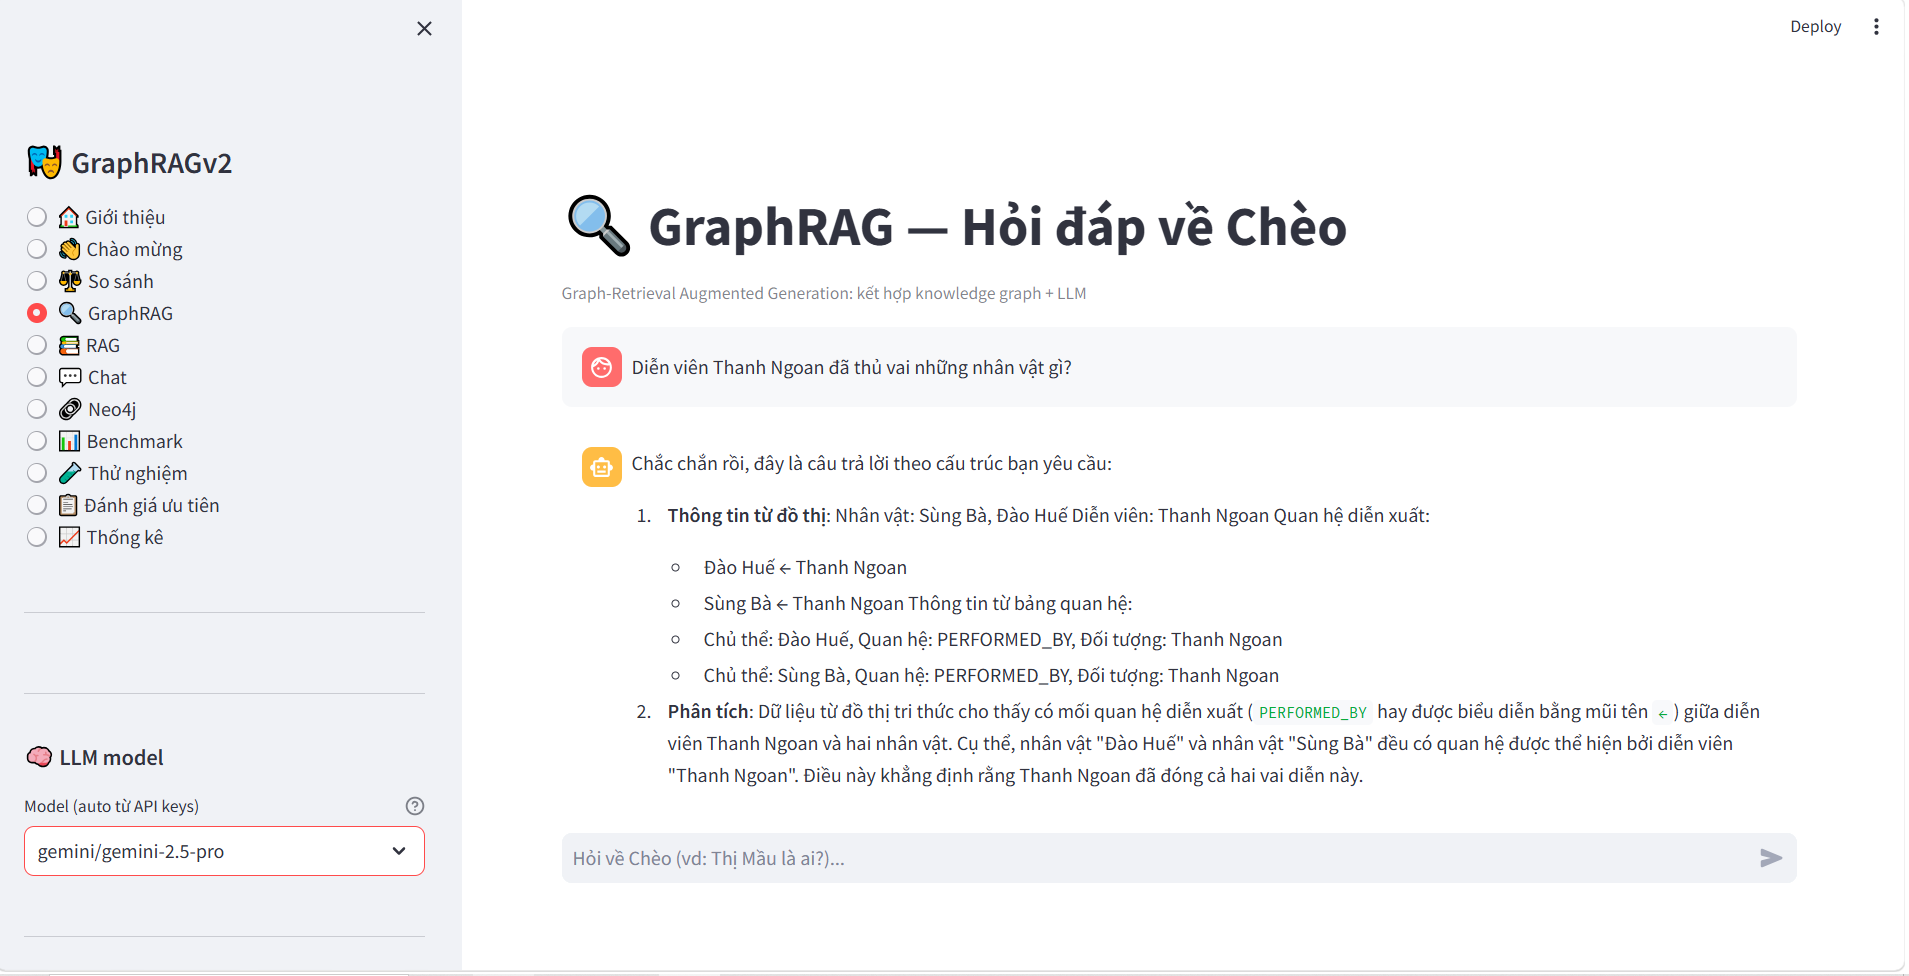
\includegraphics[width=1\linewidth]{figures//c4/UI.png}
    \caption{Giao diện hệ thống}
    \label{fig:UI}
\end{figure}

Mặc dù giao diện người dùng không phải là trọng tâm của nghiên cứu, việc xây dựng lớp tương tác này giúp kiểm chứng hoạt động của hệ thống trong môi trường sử dụng thực tế và hỗ trợ quá trình thực nghiệm được trình bày trong các phần tiếp theo.

\section{Thiết kế thực nghiệm}

Mục tiêu của thực nghiệm là đánh giá một cách hệ thống hiệu quả của kiến trúc GraphRAG được đề xuất trong việc khai thác tri thức có cấu trúc phục vụ trả lời câu hỏi trong miền nghệ thuật Chèo. Khác với các hệ thống RAG truyền thống chỉ dựa trên truy xuất văn bản thuần túy, hệ thống đề xuất tích hợp Knowledge Graph và cơ chế truy xuất đa độ hạt. Do đó, thiết kế thực nghiệm không chỉ nhằm đo lường hiệu năng tổng thể, mà còn nhằm phân tích đóng góp của từng thành phần trong kiến trúc, bao gồm chiến lược truy xuất, định dạng biểu diễn ngữ cảnh và phương pháp tích hợp ngữ cảnh vào mô hình ngôn ngữ.

Thiết kế thực nghiệm được xây dựng dựa trên ba nguyên tắc chính. Thứ nhất, nguyên tắc \textit{kiểm soát biến} (controlled variables), trong đó tất cả các cấu hình không liên quan đến thành phần đang được đánh giá đều được giữ cố định nhằm đảm bảo tính công bằng. Thứ hai, nguyên tắc \textit{đánh giá đa chiều} (multi-dimensional evaluation), bao gồm cả chất lượng truy xuất và chất lượng tạo sinh, nhằm phản ánh đầy đủ đặc trưng của hệ thống Retrieval-Augmented Generation. Thứ ba, nguyên tắc \textit{phân tích thành phần} (component-wise analysis), trong đó các thành phần của hệ thống được thay đổi độc lập để xác định ảnh hưởng cụ thể của từng yếu tố.

Toàn bộ thực nghiệm được tổ chức thành ba nhóm chính tương ứng với ba câu hỏi nghiên cứu. Câu hỏi thứ nhất là: mức độ truy xuất (granularity) ảnh hưởng như thế nào đến hiệu năng tổng thể của hệ thống? Câu hỏi thứ hai là: định dạng biểu diễn ngữ cảnh có tác động ra sao đến khả năng suy luận của mô hình ngôn ngữ? Câu hỏi thứ ba là: chiến lược tích hợp ngữ cảnh vào quá trình tạo sinh có cải thiện tính trung thực và độ chính xác của câu trả lời hay không? Ba nhóm thí nghiệm này được thực hiện độc lập nhưng trên cùng một bộ dữ liệu và cùng cấu hình mô hình nhằm đảm bảo tính so sánh.

Để đảm bảo tính tái lập (reproducibility), tất cả các thí nghiệm được thực hiện trên cùng một môi trường triển khai. Knowledge Graph được lưu trữ và truy vấn thông qua Neo4j, với cấu trúc và chỉ mục đã được mô tả trong chương trước. Mô hình ngôn ngữ lớn được sử dụng thông qua API với cùng cấu hình tham số cho toàn bộ các thí nghiệm, bao gồm nhiệt độ (temperature), top-p và top-k được giữ cố định. Điều này nhằm đảm bảo rằng sự thay đổi trong kết quả chỉ xuất phát từ thành phần đang được khảo sát, thay vì từ sự khác biệt trong cấu hình suy luận của mô hình.

Trong nhóm thí nghiệm về độ hạt truy xuất, hệ thống được cấu hình lần lượt chỉ sử dụng một chiến lược truy xuất duy nhất (node-level, triplet-level, path-level hoặc subgraph-level), sau đó so sánh với cấu hình kết hợp đa độ hạt. Các cấu hình này được thực hiện độc lập trên toàn bộ bộ câu hỏi kiểm thử, và kết quả được ghi nhận cho từng thước đo truy xuất và tạo sinh. Việc đánh giá từng mức độ truy xuất riêng biệt cho phép xác định vai trò cụ thể của từng cấu trúc tri thức trong quá trình trả lời câu hỏi.

Trong nhóm thí nghiệm về định dạng ngữ cảnh, dữ liệu đồ thị sau truy xuất được chuyển đổi sang các định dạng khác nhau, bao gồm biểu diễn tự nhiên bằng văn bản, bảng quan hệ, JSON có cấu trúc và chuỗi nút tuyến tính. Mỗi định dạng được đưa vào cùng một chiến lược tạo sinh nhằm loại trừ ảnh hưởng của các yếu tố khác. Thiết kế này cho phép phân tích mức độ phù hợp giữa cách biểu diễn tri thức và khả năng xử lý của mô hình ngôn ngữ.

Trong nhóm thí nghiệm về chiến lược tạo sinh, hệ thống được cấu hình theo các phương án tích hợp ngữ cảnh khác nhau, bao gồm tích hợp toàn bộ ngữ cảnh ngay từ đầu, hướng dẫn suy luận theo bước, và cơ chế hậu kiểm. Các chiến lược này được thực hiện trên cùng một cấu hình truy xuất và cùng định dạng ngữ cảnh tối ưu nhằm đảm bảo rằng sự khác biệt trong kết quả phản ánh đúng ảnh hưởng của phương pháp tạo sinh.

Cuối cùng, để đánh giá lợi ích của việc tích hợp Knowledge Graph, hệ thống GraphRAG được so sánh với một mô hình RAG truyền thống sử dụng truy xuất văn bản dựa trên embedding. Trong cấu hình baseline này, Knowledge Graph không được sử dụng, và truy xuất chỉ dựa trên độ tương đồng ngữ nghĩa giữa câu hỏi và các đoạn văn bản. So sánh này nhằm xác định mức độ cải thiện mà cấu trúc đồ thị mang lại trong các truy vấn yêu cầu suy luận quan hệ.

Tổng thể, thiết kế thực nghiệm được xây dựng theo hướng phân tích có kiểm soát và đánh giá đa chiều, đảm bảo rằng mỗi kết quả định lượng đều có thể được diễn giải một cách rõ ràng trong bối cảnh kiến trúc đề xuất. Cách tiếp cận này không chỉ cho phép đo lường hiệu năng hệ thống, mà còn giúp làm sáng tỏ cơ chế hoạt động của từng thành phần trong mô hình GraphRAG.

\section{Thước đo đánh giá}

Do hệ thống GraphRAG bao gồm hai thành phần chính là truy xuất tri thức và tạo sinh ngôn ngữ, việc đánh giá hiệu năng cần được thực hiện ở cả hai mức độ này. Nếu chỉ đánh giá chất lượng câu trả lời cuối cùng, không thể xác định được lỗi xuất phát từ giai đoạn truy xuất hay từ quá trình tạo sinh của mô hình ngôn ngữ. Ngược lại, nếu chỉ đánh giá truy xuất, sẽ không phản ánh được khả năng tổng hợp và diễn đạt của hệ thống. Vì vậy, hệ thống được đánh giá theo ba mức độ: chất lượng truy xuất, chất lượng tạo sinh và điểm tổng hợp.

\subsection{Đánh giá chất lượng truy xuất}

Chất lượng truy xuất được đo lường thông qua sự kết hợp giữa các thước đo truyền thống trong Information Retrieval (IR) và các thước đo đặc thù cho hệ thống Retrieval-Augmented Generation . Việc kết hợp này nhằm phản ánh cả chất lượng xếp hạng kết quả truy xuất lẫn mức độ phù hợp ngữ nghĩa của ngữ cảnh đối với câu hỏi.

Các thước đo IR bao gồm Mean Average Precision (MAP), Normalized Discounted Cumulative Gain (NDCG), Precision@K và Recall@K. MAP \cite{manning2008ir} phản ánh chất lượng trung bình của thứ hạng các phần tử liên quan trong toàn bộ truy vấn. NDCG \cite{jarvelin2002ndcg} đánh giá mức độ ưu tiên của các kết quả liên quan ở vị trí xếp hạng cao. Precision@K đo tỷ lệ phần tử liên quan trong K kết quả đầu tiên, trong khi Recall@K phản ánh mức độ bao phủ của các phần tử liên quan trong tập truy xuất.

Bên cạnh các thước đo truyền thống, hệ thống còn sử dụng các thước đo ngữ nghĩa bao gồm Context Precision, Context Recall và Context Entities Recall. Context Precision đo tỷ lệ thông tin trong ngữ cảnh thực sự liên quan đến câu hỏi. Context Recall phản ánh mức độ bao phủ thông tin cần thiết để trả lời câu hỏi. Context Entities Recall đánh giá khả năng hệ thống truy xuất đầy đủ các thực thể bắt buộc theo ground truth.

Điểm truy xuất tổng hợp được tính theo công thức:

\begin{equation}
\begin{aligned}












+
S_{\text{retrieval}} =\;& 0.20 \cdot \text{MAP} 
+ 0.15 \cdot \text{NDCG} \\
& + 0.10 \cdot \text{Precision@5}
+ 0.10 \cdot \text{Recall@5} \\
& + 0.20 \cdot \text{Context Precision}
+ 0.15 \cdot \text{Context Recall} \\
& + 0.10 \cdot \text{Context Entities Recall}.
\end{aligned}
\end{equation}

Các hệ số trọng số được lựa chọn nhằm cân bằng giữa chất lượng xếp hạng và độ phù hợp ngữ nghĩa, đồng thời nhấn mạnh vai trò của Context Precision trong hệ thống GraphRAG.

\subsection{Đánh giá chất lượng tạo sinh}

Chất lượng tạo sinh được đánh giá dựa trên hai tiêu chí chính: độ trung thực (Faithfulness) và độ liên quan câu trả lời (Answer Relevance). Faithfulness đo mức độ câu trả lời được hỗ trợ bởi ngữ cảnh truy xuất, tức là liệu câu trả lời có thể được suy ra trực tiếp từ tri thức đã truy xuất hay không. Answer Relevance đo mức độ câu trả lời thực sự giải quyết câu hỏi được đặt ra, tránh tình trạng trả lời lan man hoặc thiếu trọng tâm.

Điểm tạo sinh được tính như sau:

\begin{equation}
S_{\text{generation}} =
0.5 \cdot Faithfulness +
0.5 \cdot AnswerRelevance
\end{equation}

Việc sử dụng trọng số bằng nhau phản ánh quan điểm rằng một câu trả lời tốt phải vừa đúng với dữ liệu truy xuất, vừa đúng với yêu cầu của câu hỏi.

\subsection{Điểm tổng hợp}

Để đánh giá hiệu năng tổng thể của hệ thống, điểm truy xuất và điểm tạo sinh được kết hợp thành một chỉ số chung:

\begin{equation}
S_{\text{overall}} =
\frac{S_{\text{retrieval}} + S_{\text{generation}}}{2}
\end{equation}

Điểm tổng hợp này cho phép so sánh trực tiếp giữa các cấu hình hệ thống khác nhau, đồng thời đảm bảo rằng cả hai khía cạnh truy xuất và tạo sinh đều được xem xét. Thiết kế thước đo theo hướng đa chiều giúp phân tích rõ ràng tác động của từng thành phần trong kiến trúc GraphRAG và tránh việc đánh giá phiến diện dựa trên một tiêu chí duy nhất.

\section{Kết quả thực nghiệm}

Phần này trình bày kết quả định lượng của hệ thống GraphRAG theo các nhóm thí nghiệm đã mô tả ở mục trước. Các kết quả được phân tích nhằm làm rõ ảnh hưởng của từng thành phần trong kiến trúc hệ thống đến chất lượng truy xuất và tạo sinh. Thay vì chỉ trình bày điểm số tổng thể, các kết quả được phân tích theo từng cấu hình nhằm xác định xu hướng và mối quan hệ giữa thiết kế kiến trúc và hiệu năng đạt được.

\subsection{Ảnh hưởng của độ hạt truy xuất}

Bảng \ref{tab:granularity_results} trình bày kết quả khi thay đổi chiến lược truy xuất ở các mức độ khác nhau.

\begin{table}[h]
\centering
\caption{Ảnh hưởng của độ hạt truy xuất}
\label{tab:granularity_results}
\begin{tabular}{lccc}
\hline
\textbf{Phương pháp} & \textbf{Retrieval} & \textbf{Generation} & \textbf{Overall} \\
\hline
Nodes      & 0.46 & 0.62 & 0.54 \\
Triplets   & 0.56 & 0.70 & 0.63 \\
Paths      & 0.54 & 0.68 & 0.61 \\
Subgraph   & 0.68 & 0.75 & 0.72 \\
Combined   & 0.73 & 0.78 & 0.76 \\
\hline
\end{tabular}
\end{table}

Kết quả cho thấy truy xuất ở mức node đơn lẻ đạt hiệu năng thấp nhất, đặc biệt ở điểm truy xuất. Điều này phản ánh thực tế rằng thông tin thuộc tính đơn lẻ không đủ để trả lời các câu hỏi có yếu tố quan hệ hoặc suy luận đa bước. Khi chuyển sang mức triplet và path, hiệu năng tăng lên do hệ thống bắt đầu khai thác quan hệ trực tiếp và gián tiếp giữa các thực thể. Tuy nhiên, hai mức này vẫn bị giới hạn về phạm vi ngữ cảnh.

Truy xuất ở mức subgraph cho thấy sự cải thiện rõ rệt ở cả điểm truy xuất và điểm tạo sinh. Điều này cho thấy việc cung cấp vùng lân cận của thực thể giúp mô hình có đủ ngữ cảnh để suy luận chính xác hơn. Cấu hình kết hợp đa độ hạt đạt điểm cao nhất, cho thấy các mức độ truy xuất có tính bổ sung lẫn nhau thay vì thay thế lẫn nhau. Kết quả này xác nhận giả thuyết rằng truy xuất đa độ hạt là cần thiết trong miền tri thức có cấu trúc phức tạp.

\subsection{Ảnh hưởng của định dạng biểu diễn ngữ cảnh}

Bảng \ref{tab:format_results} trình bày ảnh hưởng của các định dạng biểu diễn ngữ cảnh đến điểm tổng thể của hệ thống.

\begin{table}[h]
\centering
\caption{Ảnh hưởng của định dạng ngữ cảnh}
\label{tab:format_results}
\begin{tabular}{lc}
\hline
\textbf{Định dạng} & \textbf{Overall Score} \\
\hline
Natural Language & 0.71 \\
Structured (JSON) & 0.72 \\
Adjacency Table & 0.68 \\
Node Sequence & 0.65 \\
All Combined & 0.76 \\
\hline
\end{tabular}
\end{table}

Kết quả cho thấy định dạng JSON và biểu diễn tự nhiên bằng văn bản đạt hiệu năng cao hơn so với bảng quan hệ và chuỗi nút tuyến tính. Điều này cho thấy mô hình ngôn ngữ hoạt động tốt hơn khi tri thức được trình bày dưới dạng có cấu trúc rõ ràng hoặc có tính ngữ nghĩa tự nhiên cao. Định dạng chuỗi nút tuyến tính đạt điểm thấp nhất do thiếu thông tin quan hệ đầy đủ.

Việc kết hợp nhiều định dạng đạt điểm cao nhất, cho thấy sự bổ sung giữa cấu trúc hình thức và biểu diễn ngữ nghĩa tự nhiên. Tuy nhiên, mức cải thiện không quá lớn so với định dạng tốt nhất đơn lẻ, cho thấy tồn tại hiện tượng lợi ích giảm dần khi tăng kích thước ngữ cảnh. Điều này gợi ý rằng cần cân bằng giữa độ phong phú của ngữ cảnh và chi phí xử lý.

\subsection{Ảnh hưởng của chiến lược tạo sinh}

Khi so sánh các chiến lược tạo sinh khác nhau, kết quả cho thấy phương pháp hướng dẫn suy luận theo bước đạt hiệu năng cao nhất trong nhóm. Chiến lược này giúp mô hình tổ chức thông tin rõ ràng trước khi đưa ra kết luận, từ đó cải thiện độ trung thực của câu trả lời. Chiến lược tích hợp ngữ cảnh toàn bộ ngay từ đầu có hiệu năng thấp hơn một chút do thiếu kiểm soát cấu trúc suy luận.

Chiến lược hậu kiểm cho thấy cải thiện nhẹ về độ trung thực, nhưng chi phí tính toán tăng đáng kể do phải thực hiện nhiều lượt suy luận. Điều này cho thấy việc thiết kế prompt hợp lý có thể mang lại hiệu quả cao hơn so với việc bổ sung bước kiểm tra sau cùng. Kết quả này nhấn mạnh vai trò của thiết kế prompt trong hệ thống GraphRAG.

\subsection{So sánh với RAG truyền thống}

Để đánh giá lợi ích của Knowledge Graph, hệ thống GraphRAG được so sánh với một cấu hình RAG truyền thống sử dụng truy xuất văn bản dựa trên embedding.

\begin{table}[h]
\centering
\caption{So sánh với RAG truyền thống}
\label{tab:baseline_results}
\begin{tabular}{lcc}
\hline
\textbf{Metric} & \textbf{GraphRAG} & \textbf{Traditional RAG} \\
\hline
MAP & 0.70 & 0.50 \\
NDCG@10 & 0.75 & 0.55 \\
Precision@5 & 0.80 & 0.60 \\
Recall@5 & 0.65 & 0.55 \\
\hline
\end{tabular}
\end{table}

GraphRAG vượt trội rõ rệt ở các thước đo xếp hạng cao như MAP và Precision@5. Điều này cho thấy việc khai thác cấu trúc đồ thị giúp đưa các thực thể liên quan lên vị trí ưu tiên cao hơn trong kết quả truy xuất. Đặc biệt trong các truy vấn yêu cầu suy luận quan hệ, GraphRAG duy trì được độ chính xác cao hơn so với phương pháp dựa trên văn bản thuần túy.

Tổng thể, các kết quả thực nghiệm cho thấy hiệu năng của hệ thống không phụ thuộc vào một thành phần đơn lẻ mà là sự phối hợp giữa truy xuất đa độ hạt, biểu diễn ngữ cảnh phù hợp và chiến lược tạo sinh hợp lý. Điều này xác nhận rằng kiến trúc GraphRAG đề xuất mang lại lợi ích rõ rệt trong miền tri thức có cấu trúc phức tạp như nghệ thuật Chèo.

\section{Phân tích và thảo luận}

Các kết quả thực nghiệm cho thấy hiệu năng của hệ thống GraphRAG không chỉ phụ thuộc vào một thành phần đơn lẻ, mà là kết quả của sự tương tác giữa cấu trúc tri thức, chiến lược truy xuất và phương pháp tích hợp ngữ cảnh vào mô hình ngôn ngữ. Phân tích sâu hơn cho thấy mỗi thành phần trong kiến trúc đề xuất đóng một vai trò riêng biệt trong việc cải thiện chất lượng trả lời câu hỏi.

Trước hết, sự cải thiện đáng kể khi chuyển từ node-level sang subgraph-level retrieval cho thấy vai trò quan trọng của cấu trúc quan hệ trong miền tri thức nghệ thuật Chèo. Các truy vấn không chỉ yêu cầu truy xuất thuộc tính của một thực thể, mà thường đòi hỏi kết nối giữa nhiều thực thể như nhân vật, nghệ sĩ và vở diễn. Khi chỉ sử dụng node-level retrieval, hệ thống thiếu thông tin quan hệ và do đó không đủ ngữ cảnh để suy luận chính xác. Việc mở rộng sang subgraph-level giúp cung cấp bức tranh toàn diện hơn, từ đó cải thiện cả điểm truy xuất và điểm tạo sinh.

Tuy nhiên, kết quả cũng cho thấy lợi ích không tăng tuyến tính khi mở rộng ngữ cảnh. Khi kết hợp nhiều mức độ truy xuất, điểm số đạt mức cao nhất, nhưng mức cải thiện so với subgraph đơn lẻ không quá lớn. Điều này phản ánh một hiện tượng phổ biến trong hệ thống LLM, đó là lợi ích biên giảm dần khi tăng kích thước ngữ cảnh. Nếu ngữ cảnh quá lớn hoặc chứa nhiều thông tin không cần thiết, mô hình có thể gặp khó khăn trong việc tập trung vào các quan hệ quan trọng.

Đối với định dạng ngữ cảnh, kết quả cho thấy mô hình ngôn ngữ hoạt động tốt hơn khi tri thức được trình bày ở dạng có cấu trúc rõ ràng hoặc gần với biểu diễn ngôn ngữ tự nhiên. Điều này phù hợp với đặc tính của LLM, vốn được huấn luyện chủ yếu trên dữ liệu văn bản tự nhiên. Định dạng quá tuyến tính hoặc thiếu cấu trúc quan hệ làm giảm khả năng suy luận của mô hình. Tuy nhiên, việc kết hợp nhiều định dạng cũng cần được kiểm soát để tránh làm tăng độ dài prompt quá mức.

Phân tích chiến lược tạo sinh cho thấy việc hướng dẫn mô hình suy luận theo bước giúp cải thiện độ trung thực của câu trả lời. Khi mô hình được yêu cầu tổ chức thông tin trước khi kết luận, xác suất sinh thông tin ngoài ngữ cảnh giảm xuống. Điều này chứng minh rằng thiết kế prompt đóng vai trò quan trọng không kém truy xuất tri thức. Tuy nhiên, các chiến lược hậu kiểm tuy cải thiện nhẹ độ trung thực nhưng làm tăng chi phí tính toán, cho thấy cần cân nhắc giữa hiệu năng và tài nguyên sử dụng.

So sánh với RAG truyền thống cho thấy lợi ích rõ ràng của việc khai thác cấu trúc đồ thị. Các chỉ số xếp hạng như MAP và Precision@5 được cải thiện đáng kể, chứng tỏ rằng truy xuất dựa trên quan hệ giúp đưa các thực thể liên quan lên vị trí ưu tiên cao hơn. Trong các truy vấn yêu cầu suy luận đa bước, RAG truyền thống thường truy xuất các đoạn văn bản liên quan rời rạc nhưng thiếu liên kết logic, trong khi GraphRAG duy trì được mạch quan hệ giữa các thực thể. Điều này cho thấy cấu trúc đồ thị không chỉ cải thiện độ chính xác truy xuất mà còn tăng tính nhất quán của ngữ cảnh.

Tổng thể, các kết quả và phân tích cho thấy kiến trúc GraphRAG đề xuất phù hợp với miền tri thức có cấu trúc quan hệ phức tạp như nghệ thuật Chèo. Việc tích hợp Knowledge Graph giúp giảm phụ thuộc vào khả năng suy đoán nội tại của mô hình ngôn ngữ và tăng khả năng kiểm soát nguồn tri thức. Tuy nhiên, hệ thống vẫn chịu ràng buộc bởi giới hạn cửa sổ ngữ cảnh và chi phí suy luận của LLM, do đó cần có cơ chế tối ưu hóa khi mở rộng quy mô dữ liệu.

\section*{Tiểu kết}
\addcontentsline{toc}{section}{Tiểu kết}

Chương này đã trình bày quá trình thực nghiệm và đánh giá hệ thống GraphRAG được đề xuất. Trước hết, môi trường triển khai và cách cài đặt hệ thống được mô tả nhằm đảm bảo khả năng tái lập thí nghiệm. Trên cơ sở đó, thiết kế thực nghiệm được xây dựng theo hướng kiểm soát biến và phân tích thành phần, cho phép đánh giá riêng biệt ảnh hưởng của các yếu tố như độ hạt truy xuất, định dạng biểu diễn ngữ cảnh và chiến lược tạo sinh.

Các thước đo đánh giá được thiết kế theo hướng đa chiều, bao gồm cả chất lượng truy xuất và chất lượng tạo sinh. Điều này giúp phân tách rõ ràng các nguồn sai lệch trong hệ thống Retrieval-Augmented Generation, đồng thời cung cấp một chỉ số tổng hợp phản ánh hiệu năng toàn diện của hệ thống.

Kết quả thực nghiệm cho thấy truy xuất đa độ hạt và việc khai thác cấu trúc đồ thị mang lại cải thiện đáng kể so với các phương pháp truy xuất đơn giản. Đặc biệt, việc sử dụng ngữ cảnh ở mức subgraph và kết hợp nhiều chiến lược truy xuất giúp tăng độ bao phủ thông tin và cải thiện độ chính xác của câu trả lời. Bên cạnh đó, các định dạng biểu diễn tri thức có cấu trúc và các chiến lược tạo sinh có hướng dẫn giúp nâng cao độ trung thực của kết quả.

So sánh với mô hình RAG truyền thống cho thấy việc tích hợp Knowledge Graph giúp hệ thống duy trì mạch quan hệ giữa các thực thể và cải thiện hiệu quả truy xuất trong các truy vấn yêu cầu suy luận đa bước. Tổng thể, các kết quả thực nghiệm xác nhận rằng kiến trúc GraphRAG đề xuất phù hợp với miền tri thức có cấu trúc quan hệ phức tạp như nghệ thuật Chèo và mang lại lợi ích rõ rệt trong việc nâng cao chất lượng hệ thống hỏi đáp.